\documentclass[9pt,oneside]{amsart}
%\usepackage{tweaklist}
\usepackage{url}
\usepackage{cancel}
\usepackage{xspace}
\usepackage{graphicx}
\usepackage{multicol}
\usepackage{subfig}
\usepackage{amsmath}
\usepackage{amssymb}
\usepackage[a4paper,width=170mm,top=18mm,bottom=22mm,includeheadfoot]{geometry}
\usepackage{booktabs}
\usepackage{array}
\usepackage{verbatim}
\usepackage{caption}
\usepackage{natbib}
\usepackage{float}
\usepackage{pdflscape}
\usepackage{mathtools}
\usepackage[usenames,dvipsnames]{xcolor}
\usepackage{afterpage}
\usepackage{tikz}

\newcommand{\hcancel}[1]{%
    \tikz[baseline=(tocancel.base)]{
        \node[inner sep=0pt,outer sep=0pt] (tocancel) {#1};
        \draw[black] (tocancel.south west) -- (tocancel.north east);
    }%
}%

\definecolor{lightyellow}{rgb}{1,0.98,0.9}
\definecolor{lightpink}{rgb}{1,0.94,0.95}

\newcommand{\firsthomesteadblock}{\ensuremath{N_H}}

\DeclarePairedDelimiter{\ceil}{\lceil}{\rceil}
\newcommand*\eg{e.g.\@\xspace}
\newcommand*\Eg{e.g.\@\xspace}
\newcommand*\ie{i.e.\@\xspace}
%\renewcommand{\itemhook}{\setlength{\topsep}{0pt}  \setlength{\itemsep}{0pt}\setlength{\leftmargin}{15pt}}

\title{RigoBlock: a Protocol for Decentralized Fund Infrastructure \\ {\smaller \textbf{ The New Paradigm For Asset Managers}}}
\author{
    Mr. Gabriele rigo\\
    Founder, RigoBlock\\
    gab@rigoblock.com
}
\begin{document}

\pagecolor{lightyellow}
%\pagecolor{lightpink}

\begin{abstract}
The asset management industry is dominated by fund distribution networks and big players. It is difficult and cumbersome for emerging managers to startup their own fund unless they have many years of experience, assets from investors and proprietary money. Yet big hedge funds scout for talent and delegate risk to very young professionals, targeting exceptional returns by exploiting the most recent research and data analysis techniques. Light operational structures exist (managed accounts) but they are burdensome to manage, require wasting a lot of time managing and rebalancing the portfolios.

Blockchain provides the ideal technology for setting up funds in a short period of time, with low setup costs and with innovations of processes which could only be imagined before. We provide the technological framework for emerging managers to set up their own investment vehicle. We discuss its design, vision of implementation and Proof-of-Concepts, the opportunities it provides in giving more transparency, efficiency to operations and innovating processes. We also propose an alternative paradigm for rewarding talent and hard work.
\end{abstract}

\maketitle

\setlength{\columnsep}{20pt}
\begin{multicols}{2}

\section{Introduction}\label{sec:introduction}

The asset management industry has been following a path of consolidation towards bigger corporate structures during the last 10 years. The hedge fund industry, in particular, has developed into a more standardized and regulated sector. High setup costs and requirements of a minimum 50 Million US Dollars or even much bigger initial Assets Under Management (AUM), automatically exclude the smaller players from the market. Reason behind such high minimum AUM requirements are high costs of providing Prime Broker services to funds: costs like Net Assets Value (NAV) estimate, collateral accounts, management company costs, legal and advisory costs. Furthermore, investment funds and management companies are in most cases no more than P.O. Boxes; by this we mean that they do not actually employ anyone, they are just offshore corporate structures.

The Ethereum protocol provides the perfect technology for creating investment vehicles on the spot, allowing subscriptions and redemptions in real time, trading on decentralized exchanges in a trust-less manner, so that no administrator or custodian is needed, allowing for a level of efficiency and transparency in the industry never seen before. One positive externality of our proposed model is that, by being agnostic of the AUM size, it is also possible it will be used as a tool to building one's track record in order to get a job at major investment funds, hence improving visibility for traders. Either way we are to lay down the path for changing how things are done in asset management.

\subsection{Driving Factors} \label{ch:driving}

Regulation is one of the main factors that often prevents fund managers to startup their own fund or forces them to consolidate with others through acquisition of smaller players, mergers, or suboptimal advisory structures which augment conflict of interests which are inherently present in the asset management industry. Scope of regulation is to monitor and manage these conflicts of interests, prevent money laundering and fraud (a manager running away with the money or inputing unjustified costs to the fund). By explaining our model we provide a framework which self-regulates by providing such level of transparency and efficiency not to require any regulation (or at least reach ultra-high self-regulation standards). The level of our structure's efficiency offers levels of compliance never seen before.

One of our main goals is to provide every single individual with the possibility of seamlessly creating/deploying their own investment vehicle. Our vision is to provide the technology for people to be able and express their talent, share their passion and compete globally without having any access to investors' funds other than for trading. This reduces the amount of work on the operational side of the business, leaving the manager with no other focus than producing good risk-adjusted return for their investors.

Conflicts of interests are often one of the reasons for funds' poor performances, and in many ways and with many mental biases (myopic loss aversion, inability to replicate exceptional returns when AUM increase dramatically) may lead to poor performances. In some cases it even leads good managers to quit funds they are working for and retire, once they are tired of the continuous conflicts of interests within such structures. We believe that completely erasing conflicts of interests is in the best interest of both the investors and managers.

Overall, we wish to provide a completely decentralized framework that puts the manager first and offers investors the best-in-class technology, aligning their mutual interests. Furthermore, we aim at creating a competitive, transparent and meritocratic market for talent.

Most of the blockchain models for asset management proposed by others so far have a highly centralized approach, therefore requiring a level of trust to relatively unregulated entities.

\subsection{Market Overview} \label{ch:previous}

Although currently we haven't seen any asset management platform built on the blockchain, we have to recognize previous attempts in the field of trading and asset management.

The Stellar network provides a platform for issuing tokens which have been used for trading, streamlining the share issuance, subscription and redemption phases, but still requesting trust of the users since its approach is centralized and the subject issuing tokens is in total control of the assets.

The Iconomi project aims at being a platform for crypto-related-assets trading, digitizing processes of share issuance, subscriptions and redemptions with a \textit{centralized server-based approach}. They provide a user-friendly front-end platform which does not require interaction from blockchain browsers. They are the funds' custodian (now partner with a regulated UK asset manager in order to provide the technology and liquidity stack only) as they manage a user’s private key, thus requiring some level of trust in their infrastructure. The platform is aimed at professional managers. The RigoBlock technology, in the context of companies like Iconomi, can be seen as a decentralized engine which could be easily plugged-in in order to create the funds on-chain.

The first attempt to formalize a decentralized approach to private banking has been proposed by a project named EtherPlan. Still the idea required a high level of trust and substituted many of the existing frictions with new, more technologically advanced ones, thus not being able to pose the fundamentals for a radical change, at least in these early stages of the \textit{development of the technology}. The project is currently on stand-by. A similar approach has been recently adopted by the Swissborg project, which itself can be seen as a potential customer.

The first attempt of using blockchain technology in a \textit{completely decentralized form} is Melonport, a project which was chronologically born at the same time as our first concept Drago the decentralized hedge fund, now RigoBlock Drago. Both our protocols aim at solving the same problem, but with different methodologies; they can be seen as our closest competitor, even though at such early stage of technology the two projects might also be seen as complimentary to each other. Melonport also provided the first formal specification for the technological framework and the concept of an open protocol for decentralized asset management, leveraging and relying on external developers to deliver some of their "modules". RigoBlock applies the same concept in a more abstracted and liberal way, so that developers can "bring their own asset management version" and leverage our protocol.

Prism, by Shapeshift, is a dual product, being at the same time a decentralized exchange and a hybrid asset management platform. Prisms are the equivalent of financial structured products built on the blockchain (for who is familiar with structured products). Prism is still in closed-alpha testing. For RigoBlock, Prisms can be treated as assets tradeable by our decentralized pools of tokens (the Dragos).

At the current state of the art, however, no asset management platform has been brought to life on the Ethereum main network. Much of the reason being that decentralized exchanges themselves now exist only in form of alpha and on the \textit{test networks}. A few questions are still unanswered and we will try to address them in the following paragraphs, although very humbly we state that the answers are yet to be found and the directional path of the different projects will be decided by their management and by the advance in technology as well.

%E language?

\section{Blockchain and Funds}\label{ch:conventions}

In order to explain the process of creating a fund on the blockchain, we recall the concept of \textit{Smart Contracts}. Smart Contracts allow for coding the dynamics that manage a particular process directly into the blockchain, segregating the creation process and its management from anything else, isolating it by creating a unique code, a unique hash of the transaction and a unique hash of the transaction each time a function is called from the code deployed on the blockchain. This means that potentially anyone can use the same \textit{Solidity source code}\footnote{Solidity is a native Javascript-based language of the Ethereum blockchain, it is used to completely segregate the code of everything related to the back-end (blockchain) from everything else).} to create vehicles that are identical by nature but have their own unique identifier code, and that can be personalized to different predefined extents, each one corresponding to a different level of trust required by the platform, starting from a completely trustless environment, to more trust-reliant ones.

\subsection{The Trust Factor} \label{ch:transaction}

Exchanges of value occur on the blockchain without requiring the counterparts to trust each other. This is the beauty of blockchain technology, and the good thing is that it can be ported to smart contracts as well. The strict use of \textit{escrow accounts}, in fact, allows for the transfer of money within the fund to happen in a trustless way.
More in detail, we state that once some amount of value is in the fund, that amount can only be used for trading purposes by the manager, who never has access to it. The manager can only instruct a deposit to an escrow account of a decentralized exchange: money never leaves the blockchain and is always under control of the fund; neither the manager nor the platform at any time may access those funds. \textit{Immutability} is the great property of the blockchain that makes it possible to trust that the code will forever do only what it is programmed to do, and nothing more.

\subsection{The Drago Creation} \label{ch:block}
Dragos are the way we call our funds, aka decentralized pools of tokens. The RigoBlock platform is currently in alpha, accessible in the Parity DApp store and visible globally by users locally running the Parity UI; this consists of running a software (the Parity client) in the background and accessing the store through a normal web-browser interface. You can find RigoBlock on the "Applications" tab, and you will be able to use it if you are running Parity on the Kovan testnet. We also offer a view-only alpha web version accessible at pool.rigoblock.com and an IPFS DApp at rigo.network.
The decentralized pools of tokens are created by clicking one button on the application, and the platform takes care of deploying the code on the blockchain through one transaction. By inputing a name and a symbol for the fund, a pop-up requires the user to execute the transaction. As soon as the transaction is mined, the user is able to see the new fund created and anyone can immediately subscribe shares of the fund through an automatic token minting process. When a user has a positive balance of shares, she can redeem her shares for Ether by executing the opposite transaction, thus burning tokens and receiving Ether in exchange.
Our approach has been to implement the software completely on-chain, therefore creating a trustless environment and a serverless backend infrastructure. Functions like NAV calculation, however, will be performed off-chain, thus using the blockchain in its most efficient and effective way. We care to stress out that everything concerning transfers of titles and money happens on-chain and in a decentralized manner, therefore all the functions related to the existence and behavior of the decentralized funds are audible in real time and by anyone just by knowing the code of the fund, not having to trust information provided by us.

\section{Social Trading} \label{ch:create}
Often do we hear that fund managers must have their investments undisclosed because otherwise competitors would be able to copy their positions and they would not be able to exploit market inefficiencies. We propose two different objections to the open question. The first one is the observation that \textit{Social Trading Platforms} which force managers to have their portfolios public have experienced enthusiastic participation of managers. The second objection is based on a regression of financial markets in general and their efficiency: through a radical shift in the concept of secrecy, therefore mirroring in finance the (relatively) novel approach of open source software development, we envision the possibility of information getting reflected in market prices more efficiently. The manager will be rewarded for performing her research job based on the concept of meritocracy. We feel the urge to testify that inefficiencies/anomalies are in the market for a long period of time normally. Furthermore, the very reason of the existence of financial markets is that people disagree on the same subjects. In most cases it is equally skilled money managers that have different models for analyzing data, which give opposite output by analyzing the same input factors. In other cases it is professional managers against the \textit{amateurs} (uninformed players). To the most extreme cases, it is a group of professional managers against politicians (a central bank or a government). In any case people disagree and individuals live constantly in a prisoner's dilemma, where a rational expected behavior is often not empirically observed.
We hope our work can serve to drive financial markets towards the path of efficiency, even though we realize the beauty and complexity of the human mind, especially when it comes to managing money, leads us to make mistakes that are objectively irrational when analyzed in hindsight.
If our work can help the average investor in getting good returns on her financial portfolio by delegating management to those professional managers, we believe we will have made a difference.

\section{A Dashboard For Trading} \label{ch:model}
One of our goals is to provide an integrated set of tools for trading, which goes from front-office execution to back-office reconciliation. Therefore, we also want to integrate the platform with a section dedicated to an off-chain dashboard for the portfolio, with statistics about performance on different time frames, display of positions in the portfolio and possibility of visualizing all trades relative to every single position; monitoring of risk, evolution of portfolio risk over time. These are all very powerful tools that are normally available for professional manager, not so much for small or emerging managers. This is the path going forward in the evolution of the platform.
We are working to deliver Javascript libraries which allow automated quantitative trading strategies through our APIs and easy interface with other front-end platforms.
Thanks to our modular architecture, external service providers can build their own Dashboard on top of our protocol, or even create their own forked version of a decentralized asset management platform using just some of our modules, leveraging our protocol and the Rigo token (alternatively called GRG token) incentives mechanism.

\section{NAV estimate} \label{ch:ghost}

Assets never leave the blockchain, hence it is pretty straightforward to track them. Further to that, accounts and positions are available in real time and balances are updated in real time automatically. This means that no more a person from the fund's operations will have to manually reconcile the position with a fund's front-office and the prime broker's back-office. No more mistakes or typos: when a trade is executed from the front-office, it is also automatically reconciled in real time on-chain, so that anyone can audit it. This allows, potentially, to estimate NAV in real time.
Since NAV estimate and registration on-chain require the use of computation of the \textit{Ethereum Virtual Machine} (EVM), we decided to provide an off-chain NAV estimate in real time to the users. The user will then update the official NAV price on the Blockchain only when needed, hence not wasting unnecessary computational and storage resources. We create a mechanism of incentives to provide the conditions for honest behavior: instead of relying on an external \textit{Oracle} to provide a NAV estimate, it is the manager herself that published the price.

\subsection{Fair User Behavior And NAV Publishing}
According to our approach, the user will publish a bid and an ask price for the shares of her fund. At those prices the fund is forced to buy and sell any amount of the shares. Therefore two conditions have to be met all the time: the fund has to always keep a minimum amount of Ether available for redemptions, in order to be able to fulfill requests in real time; the manager will have to publish the actual NAV value, otherwise becoming potential target of arbitrageurs.
The educated reader might think that manipulation and dishonest behavior are factors which should not be taken out of the equation, since at the end we are all humans. One possibility is to have the code sorting out everything for us, which is a viable approach and we will consider further developing towards this path. Our current alternative is to create a mechanism of incentives, where good behavior is rewarded and bad behavior is punished, so that NAV estimate does not rely on a centralized party. First of all, the whole infrastructure is built in a transparent manner, so that all information is public; even if NAV estimate is not performed on-chain, each individual has the possibility of performing a due diligence of the portfolio in real time. Second, by allowing good managers to access a market of "Fund of Funds", we lay down the basis for honest behavior and exponential growth for the best managers.
Lastly, we would like to remind that one of the most important references in a trader's career is her own track record: either NDAs with previous employers or the use of single managed accounts make it difficult to provide an actual track record. Auditing by a third party is also quite expensive. With our proposed paradigm, an audited real time track record obtained by trading real money is not only available through the NAV published by the trader, but also computable by anyone requesting the data directly from the blockchain, therefore without requiring any friction or intermediary. The world-famous American financial journalist and trader Jack D. Schwager has recently launched a startup for performing these calculations and audits on traders' traditional managed accounts, as a proof of need of such product.

\section{Rewarding Performance}
Many investors, amongst which legendary investor Warren Buffett, have publicly criticized the risk-taking culture in asset management and hedge funds in particular, which is enhanced by the current fee structure. In fact the typical 20 percent performance fee is criticized for pushing managers to take too much risk focusing on short term performance. The presence of hefty management fees in most cases leads to big funds' lackluster performance. An empirical phenomenon observed with the growth of a fund is the inability to replicate exceptional returns obtained in the early days. At that point their management fees are so high that are often not justifiable based on the cost structure of the hedge fund.

\subsection{A New Way Of Aligning Interests}
What we propose is a radical change in the way performance is rewarded, whose reason behind is twofold: on one side, we aim at improving the quality of management; on the other side, while the calculation of management and performance fees on-chain can result expensive, our model exploits one key characteristic of blockchain technology which makes it ultra-easy to calculate a fee per each transaction and automatically allocate it to the correct account without need of manual reconciliation or settlement.
Rather than a management and performance fee being charged to the fund directly, our protocol has no fees, and managers get rewarded in Rigo tokens thanks to an algorithm called Proof-of-Performance, which is built on top of the protocol.
The Proof-of-Performance module computes the assets and the performance of a fund for each sub-period and rewards the traders, on a quarterly basis, based on those two factors. At the end of each period, a trader can claim her reward.
The Proof-of-Performance algorithm's parameters are set by the Rigo token holders, so that they can decide on the fair reward ratio.

\subsection{Distribution}
A further way to create an ecosystem for funds is the concept of distribution: third-party platforms can leverage our module \textit{Distribution}, or create their own one on top of our protocol, and set a per-transaction fee, which is to be set and modified arbitrarily by the distributor, but publicly available. The distributor therefore transparently sets her own fees in a competitive market. While normally the use of this type of fee is prone to manual errors (either calculation or settlement), through the use of blockchain, this is performed automatically and seamlessly. The amount of work for a traditional management company for such operations makes this procedure today very expensive to execute.

\subsection{Excessive Risk Taking}
Excessive risk taking is the practice of exploiting a 20 percent performance fee by taking as much risk as possible in order to generate the biggest returns, therefore allowing the manager to focus on short term gains. We believe that our Proof-of-Performance model has the potential to shift management focus more on the long term, while at the same time leaving uncapped the total amount a good manager can receive, as the Rigo token holders can together set the correct parameters for rewarding performance. We believe, in the long run, this methodology will not lead to lower pay for the manager, but since her focus is on long term returns, it will improve the quality of the returns.


\section{Vault} \label{ch:minimum}
By removing most of the hypotheses set before, the resulting product is a completely trustless and simple vehicle: the Vault. It can be seen as  \textit{trustless version of Xapo for the Ethereum community}.
Xapo is a service that allows safe Bitcoin storage for individuals and institutional clients. It allows the creation of as many accounts as needed with each account having an ultra-secure Bitcoin storage vault. They provide a centralized service and have access to clients' keys, ultimately to clients' assets.
We think different: we want our service to be totally decentralized, and never have access or knowledge of clients' keys. It is ultimately the client who is responsible for her own keys. In order for the service to be totally decentralized and trustless,  a Smart Contract is coded in order to only allow the exchange of Ether for tokens, minting tokens to the sender of Ether and burning tokens sent in exchange for Ether. It is a distinctively different approach from Xapo's ultra-secure cold-storage, and it is made simple by the possibility to code the functions that rule the transfers directly on-chain and secured by the design of the smart contract. With our approach, no matter what, the client is always in control of her assets. Furthermore, since the code is deployed on-chain, no matter what happens to the company running the platform, the code will always allow the owner of some tokens to redeem them for Ether, thus resulting fraud and censorship proof.
By design, our product becomes the technology layer which can be potentially used by services like Xapo (i.e. cryptocurrency wallets) for offering safe Ether hot-storage and at the same time allowing for key cold-storage: keys can be off-chain, but at the same time a user can query the blockchain to visualize in real time the total deposits and for each user.
First hypothesis we relax is the possibility for the manager to transfer to escrow accounts: they are no more possible; we prevent any transfer of Ether from within the fund. In this case the manager cannot even transfer Ether to an escrow account.
Second hypothesis we relax is NAV estimate. In this case NAV is fixed at 1 Ether per share. Since the fund only holds Ether, does not have any management or performance fees, the value of one share will always be the same. Now we have a product which one can use to create her own decentralized pool of tokens, buy tokens in real time at a known price, sell tokens in real time at a known price. She can create as many funds as she wants, thus having an efficient tool for managing her family and friends or even institutional investments. She can even set a transaction fee each time tokens are bought, and receive it automatically without need to reconcile with a third party or spend time on calculating fees.
Vault is a product aimed for anyone looking to securely store Ether in one place, who have more or less experienced the same problem: holding Ether on behalf of others and bearing all the responsibility for it, plus being able at any time to access those funds, as the Ether is bought and held for the long run.
Vault is our first product to go live to the Ethereum mainnet, as it leverages the RigoBlock protocol and the Proof-of-Performance incentives mechanism, but does not rely on external services being operational (decentralized exchanges or oracles). Current work on our Vaults has been on pre-setting it to interact with Casper, the next frontier in Ethereum-based mining, in order to allow for pooled Proof of Stake mining. Our Vaults are expected to go live on the Ethereum mainnet during Q3 2018 and pooled Proof-of-Stake mining could coincide with Ethereum Constantinople (the migration of Ethereum to Proof-of-Stake, Q4 2018).

\section{RigoBlock Registry}
The RigoBlock Registry is similar in nature to the ENS (Ethereum Name Service) and allows approved asset management companies register their funds on-chain and be able to interact with their funds by the use of the name of the funds, rather than the HEX address currently needed to make transfers on-chain. We have split the RigoBlock Registry as a separate component to facilitate use from external parties. We are really looking forward for external service providers to leverage on our modular infrastructure, as rather than creating and managing their own registry, they can just plug into our Registry application and interact with.

\section{RigoBlock Exchange}
The RigoBlock Exchange has been built with the purpose of providing a decentralized exchange for the Dragos to trade. It is a completely decentralized exchange for leveraged cryptoswaps trading. It allows users to place a leveraged (or not) trade on ETHUSD (just one asset on the exchange at the moment) both on the long and on the short side, so that traders can profit if the price goes up by buying, but also on selling the position short. A derivative is a contract that represents an asset which does not exist on the blockchain.
The RigoBlock Exchange is limited by the challenges all decentralized exchanges face today (mostly slow execution, aka latency, and gas fees for unexecuted orders) but it is one of a kind, and we are looking forward to improve it, as we believe that decentralized exchanges are the new frontier of financial trading. The RigoBlock exchange is a long-term project and we are not looking to put it in production soon, as current work is on integrating decentralized exchanges with our Dragos.

\section{Proof-of-Performance}
Proof-of-Performance is our new paradigm for rewarding managers’ performances. As we said before, we disrupt the traditional concepts of management and performance fees. Proof-of-Performance allows traders to mine (technically mint) GRG tokens based on their risk-adjusted performance. The bigger their pool of tokens, the more GRG tokens they will be entitled to mint. Managers are required to hold a minimum amount of GRG tokens in order to run their own decentralized pool of tokens.
The GRG token does not hold intrinsic value, is not represented by any real activity or security, does not bear or entitle to any dividends or interest is not backed by assets. Its sole purpose is for allowing reward of performance of traders and being at the basis of our incentives mechanism.

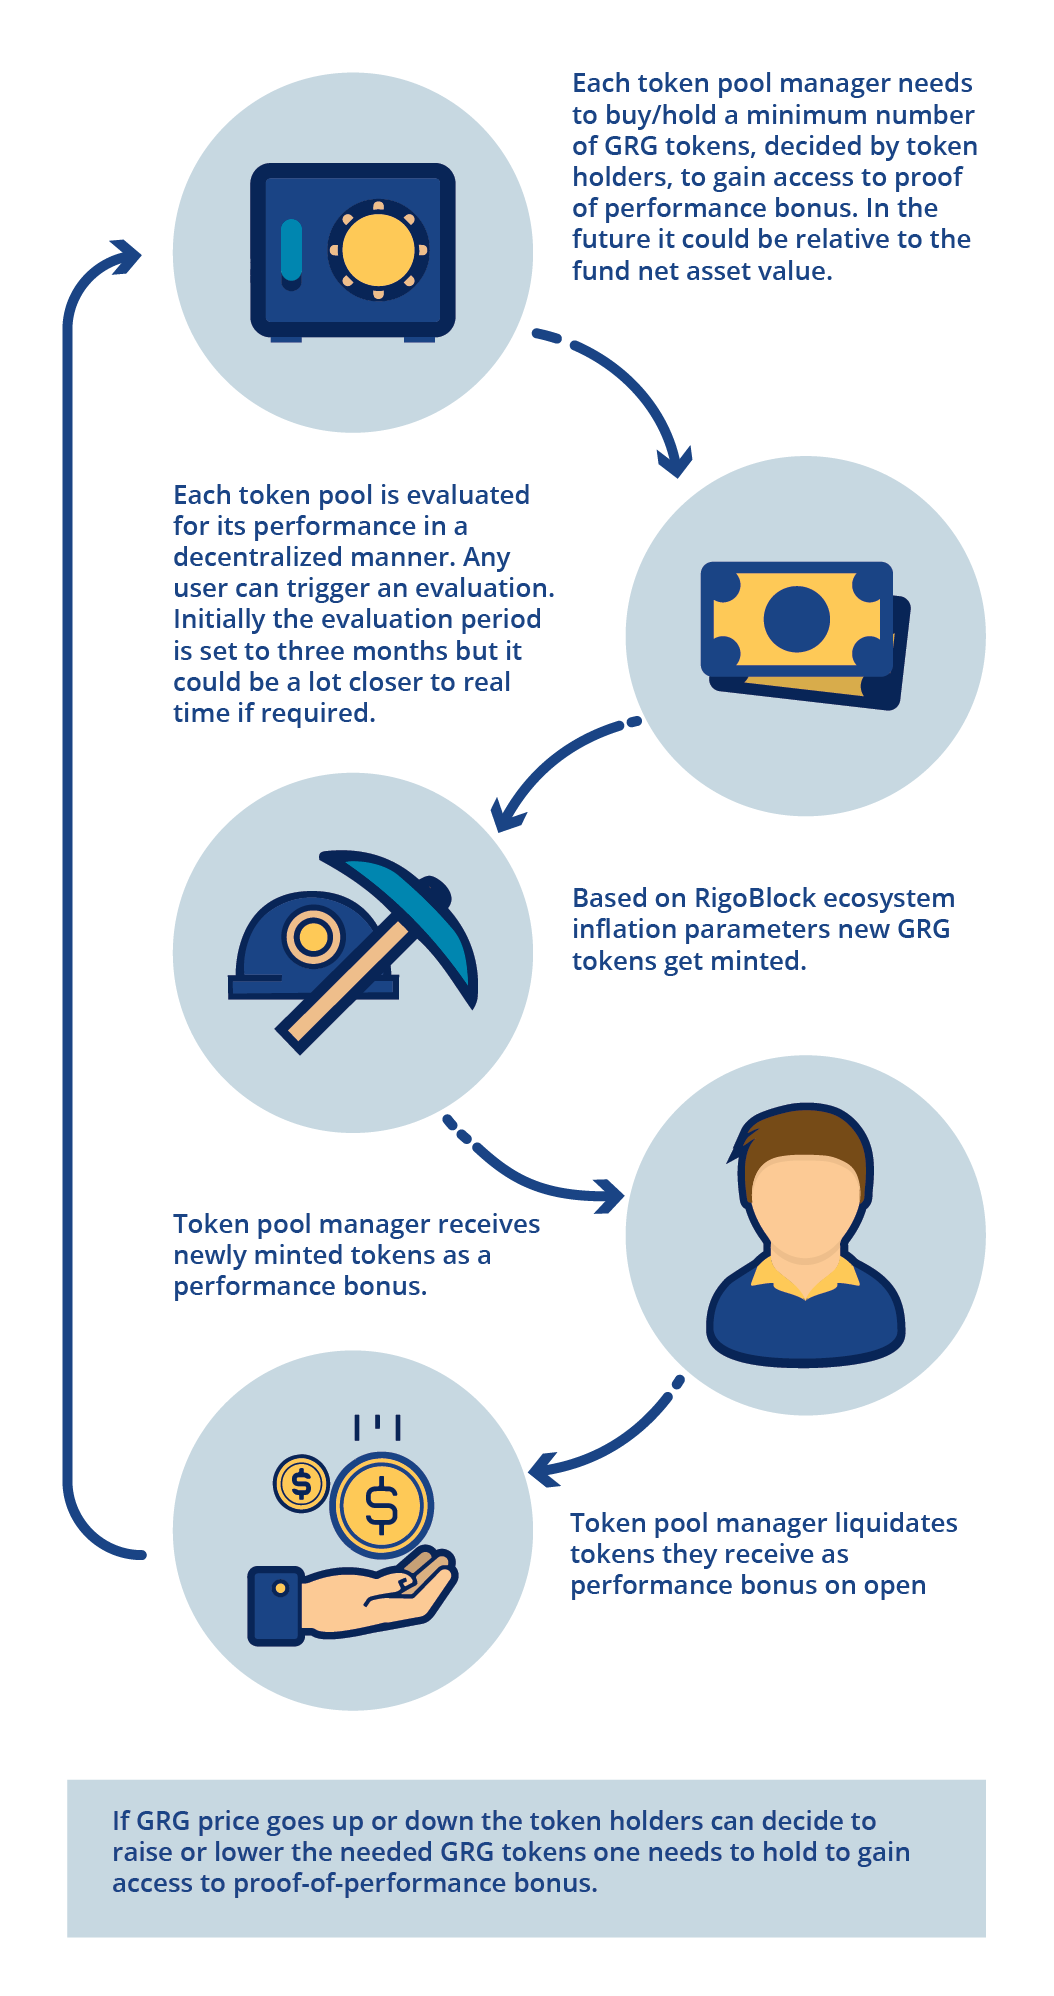
\includegraphics[width=8.2cm]{pop-tokenomics.png}
The above picture is a summary schematic of the Proof-of-Performance incentives system. This shows token pool managers receiving rewards based on the condition they hold the minimum amount of GRG tokens in their own wallet. Standard users are also required to hold GRGs in order to unlock premium features, which are otherwise locked by default. 

In particular, activities which might require the status of ”accredited”, ”specialized”, or which might fall under the scope of regulation, will require users to hold minimum thresholds of GRG tokens.

\subsection{The Assets Component}
The first component of the Proof-of-Performance reward is the size of a token pool. The amount of new GRG tokens for the token pool manager is proportional to its assets. It is a substitute for traditional management fees. 

\subsection{The Performance Component}
The second component is a calculation of the absolute performance of a token pool in respect to the previous observation period.  This is a quarter of a year by default, however, can be adjusted to allow for shorter or longer time frames.

\subsection{The High-Water Mark}
Each token pool gets benchmarked against its high-water mark, ensuring that only positive performance is compounded. Unless a token pool’s net-assets-value is at least equal to its high-water mark, no Proof-of-Performance tokens can be minted for said token pool.

\subsection{Dynamic Parameters Setting}
The assets and performance components are combined in a dynamic way set by the token holders, so that market equilibriums determine the optimal mix. Each manager’s reward is obtained by multiplying the assets and performance components combined by the reward factor of the class (or application) the token pool belongs to. The reward factor is dynamically set by the token holders. 

This new paradigm shift moves token pool managers’ rewards from the traditional management and performance fees, to a bonus awarded by the network. This is then paid in the form of a moderate inflation (expected aggregate between 1 and 2 percent), which has the benefit of attracting users as well as external developers to the RigoBlock ecosystem. 

The Proof-of-Performance incentives system, to sum-up, rewards the managers in case of non-negative performance. Which in turn, creates an incentive to bring assets into the RigoBlock ecosystem, rather than keeping them in standalone applications.

\subsection{The Components of Demand and Offer}
The GRG token is an inflation token. New tokens get created and allocated automatically by the Proof-of-Performance algorithm, enforced by smart contracts. The new tokens then get distributed to the token pool managers. 

Such a reward is a substitute to management and performance fees. The distribution happens automatically from the Proof-of-Performance module tied to the GRG token, in a fully auditable and transparent way, and without manual intervention or reliance on a centralized counterpart. 

The managers must hold a minimum amount of tokens in order to receive their rewards. The minimum is dynamic and set by the token holders, so that the ratio between inflation and demand within the ecosystem will be balanced. Standard users will be required to hold some GRGs in order to unlock premium features of the platform, thus generating additional demand. 

The RigoBlock protocol retains a royalty of 5 percent of new tokens created, in order to generate a continuous funding model which allows the reward of external developers creating applications on top of the RigoBlock protocol. Since the GRG token holders set the inflation parameters, the continuous funding model provides them with an incentive of targeting a positive inflation, rather than a null new tokens generation.

\section{Future Directions} \label{ch:future}
We have been building our proof of concepts since early 2016, with our first smart contracts for a decentralized investment vehicle released around August 2016; ever since we have been working on improving our concept, adding functionalities, checking for security and making the code a modular protocol, what we call the “smart contracts engine” so that it is more abstract and allows external service providers create their own decentralized management company on top of RigoBlock. Our platform has gone through alpha testing on the Kovan testnet and publicly accessible within the Parity UI since May 2017. We have made such choice to allow testing in a safe environment before moving to a more traditional UX experience.
Substantial work has been done on improving UX/UI and the platform has been upgraded to a beta in Q1 2018, accessible from the web. A selected group of early-testers is currently using an advanced beta. Our team has already expanded substantially, with a team of more than 10 people now (three of them are advisors with relevant experience and competencies in the field of asset management, legal, crypto/blockchain), an improved interface and a more easily-accessible platform to the average user.
During the last few months substantial progress on decentralized exchanges has been made: the 0x Protocol is setting a standard for efficiently using blockchain for creating hybrid decentralized exchanges and many \textit{relayers} are already building on top of it, bringing institutional liquidity to decentralized exchanges. Further to that, 0x upgrade to allow for fund interaction is expected to go live on the Ethereum mainnet during mid-late Q3 2018.
Our Dragos have already been integrated and tested with the RigoBlock Exchange as to demonstrate our PoC. At launch, our Dragos will only be able to operate with limited functionalities and, projected Q4 2018, external exchanges will be connected to the protocol.
The RigoBlock Exchange is reliant on external oracles and will not go in production if we can find a better decentralized exchange for derivatives. We are also cooperating for work on decentralized oracles systems, which will reduce the cost of maintaining on-chain oracles. This is more of an optimization work as we have built our own oracles and are looking for an efficient way to provide free prices for everyone.
Our ultimate goal, once our technology is fully operational on the Ethereum mainnet, is to make the RigoBlock platform an ecosystem for traders, allowing any investment strategy, no matter how twisted or strange, be performed. One of the tools for creating such ecosystem will be to allow funds invest into other funds (dedicated fund-of-funds structures) and build autonomous pools of funds whose task is to invest in the best trading strategies and be able to more easily raise from the crowd thanks to its unprecedented level of diversification. Such pool-of-pools will have the power to levy the traders from the burden of regulation as the RigoBlock pool, in this case, will act as a global traders’ fund with thousands or potentially millions of traders and bear all regulatory costs, acting as a guarantor.

\subsection{Third-Party Integrations}
Our modular blockchain solution allows an existing marketplace to offer their own funds on their own platform or wallet application. Third-parties can offer funds by interacting with our Javascript APIs. As we do not have access to the funds' assets and do not manage or have access to the keys, third party platforms can focus on managing the keys of their users and integrating their existing services, either under our brand or under their own brand, at their own choice. They can charge fees on top of our protocol, and, thanks to our \textit{Distribution} module, they can charge distribution fees.

\subsection{Decentralized Governance}
One peculiar topic could be the possibility of fraud. What if a scam-token got listed on an external decentralized exchange and bought by the same creator through a decentralized pool of tokens deployed on our platform? We have already addressed this question by creating an \textit{Authority and Governance mechanism} which allows trading only to an approved trader, from approved pools of tokens, to approved exchanges and even the tokens of the exchanges have to be approved. This has been created to improve compliance of the RigoBlock ecosystem. While this might be seen as a limitation of decentralization, it is future-proof and upgradeable, and it is the Rigo token holders that set the parameters for the decentralized governance, with the vision that RigoBlock, over time and when the technology allows for safe decentralized governance, will become a completely decentralized organization.

We share the vision that \textit{the world's value is becoming tokenized} and we aim at becoming the reference tool for organizing the value: tokens and tokenized assets. We envision stable-currency-denominated funds and share classes (hedged and unhedged). Long term we envision a world where everything related to money is transacted through the blockchain, different protocols communicate with each other, salaries and taxes are paid using digital tokens. So far the only imaginable way of providing a blockchain-agnostic framework has been to have a centralized approach with a centralized intermediary taking care of the different blockchains and transfers from one another. Notable projects are proposing a solution through the use of side-chains (Hyperledger) by making use of relayers (BitcoinRelay) and, last but not least, Polkadot, which proposes the use of validators for allowing all blockchains to be aware of what the other blockchains are doing and thus allowing transfers from one chain to another, be them the public blockchain or private or consortium ones.

\subsection{Scalability}

Scalability of the platform will be directly connected to the scalability of the blockchain it is built on. Further to that, decentralized storage for the application will provide a cost effective and infinitely scalable solution to DDoS attacks and it will result in the platform being censorship-resistant.
Swarm, the decentralized storage solution for Ethereum, and IPFS provide such a solution.
At last, the fund structures are as scalable as the markets that are traded; a manager has immediate visibility and global reach, therefore eliminating national boundaries. The proposed Fund of Funds structure allows for professionally scaling the business and possibly even choosing to target \textit{institutional clients} only.
Scalability is one of the current limits of \textit{social trading} when applied to real money. By that we mean that a trader with a lot of followers might not be aware of the price impact on the price her trades have; in case she is aware, there is even the possibility of free riding her own clients, therefore totally dis-aligning their common and individual interests. RigoBlock Drago, by contrast, provides a highly scalable infrastructure where trading is as scalable as the markets a manager trades. Further to that, a trader has all the benefits of pooling investors together without the need of periodic rebalancing of single accounts.
Ultimately, the topic of regulation will be responsibility of the individuals using the RigoBlock protocol. Pooling investors' clients is subject to regulation in most countries under certain conditions. Regulation differs according to target clients and business models; in some instances it is very limited, in others it is burdensome. What we propose is a framework which automatically self-regulates and poses higher guarantees of compliance than traditional fund structures, thus much alleviating the work needed in operations. Under certain conditions, we believe some of the managers might be completely out of reach of the scope of regulation, as with our proposed pool-of-pools model. Our job is to provide individuals with the technological tools to efficiently do their job, and to focus on their core business. Creating an ecosystem for trader, for us, means solving their problems one by one.

\section{Conclusion} \label{ch:conclusion}

We have introduced, discussed and formally defined the RigoBlock protocol. Through our Smart Contracts Engine, a trader may deploy a decentralized pool of funds on the RigoBlock platform on the Ethereum network and immediately she or her investors will be able to subscribe or redeem the shares of the fund in real time. Contracts are autonomous and immutable, the manager can only manage them. This level of transparency, efficiency and accountability constitutes a self-regulatory body never seen before in any regulated environment. We propose a different paradigm for rewarding performance through Proof-of-Performance, a new token minting algorithm.

\section{Acknowledgements}
We might not be able to give proper acknowledgement to all the people that gave us feedback and helped us improve over time. A special thanks goes to Ms. Hanna Keskin, Mr. Sharif Tarver and Mr. David Fava for providing valuable feedback on this work and to Mr. Mikko Ohtamaa for helping explain the Proof-of-Performance system in a visual and clear way. Thanks to the Ethereum community for creating an open architecture for us to be able and execute our vision and to the Parity team for all the tools built for the community. Last but not least, thanks to our testers: we are working hard to improve your experience on the RigoBlock platform.

\end{multicols}

\end{document}
